\documentclass[11pt,a4paper]{report}
\usepackage[textwidth=37em,vmargin=30mm]{geometry}
\usepackage{calc,xunicode,amsmath,amssymb,paralist,enumitem,tabu,booktabs,datetime2,xeCJK,xeCJKfntef,listings}
\usepackage{tocloft,fancyhdr,tcolorbox,xcolor,graphicx,eso-pic,xltxtra,xelatexemoji}

\newcommand{\envyear}[0]{2025}
\newcommand{\envdatestr}[0]{2025-04-19}
\newcommand{\envfinaldir}[0]{webdb/2025/20250419/final}

\usepackage[hidelinks]{hyperref}
\hypersetup{
    colorlinks=false,
    pdfpagemode=FullScreen,
    pdftitle={Web Digest - \envdatestr}
}

\setlength{\cftbeforechapskip}{10pt}
\renewcommand{\cftchapfont}{\rmfamily\bfseries\large\raggedright}
\setlength{\cftbeforesecskip}{2pt}
\renewcommand{\cftsecfont}{\sffamily\small\raggedright}

\setdefaultleftmargin{2em}{2em}{1em}{1em}{1em}{1em}

\usepackage{xeCJK,xeCJKfntef}
\xeCJKsetup{PunctStyle=plain,RubberPunctSkip=false,CJKglue=\strut\hskip 0pt plus 0.1em minus 0.05em,CJKecglue=\strut\hskip 0.22em plus 0.2em}
\XeTeXlinebreaklocale "zh"
\XeTeXlinebreakskip = 0pt


\setmainfont{Brygada 1918}
\setromanfont{Brygada 1918}
\setsansfont{IBM Plex Sans}
\setmonofont{JetBrains Mono NL}
\setCJKmainfont{Noto Serif CJK SC}
\setCJKromanfont{Noto Serif CJK SC}
\setCJKsansfont{Noto Sans CJK SC}
\setCJKmonofont{Noto Sans CJK SC}

\setlength{\parindent}{0pt}
\setlength{\parskip}{8pt}
\linespread{1.15}

\lstset{
	basicstyle=\ttfamily\footnotesize,
	numbersep=5pt,
	backgroundcolor=\color{black!5},
	showspaces=false,
	showstringspaces=false,
	showtabs=false,
	tabsize=2,
	captionpos=b,
	breaklines=true,
	breakatwhitespace=true,
	breakautoindent=true,
	linewidth=\textwidth
}






\newcommand{\coverpic}[2]{
    % argv: itemurl, authorname
    Cover photo by #2~~(\href{#1}{#1})
}
\newcommand{\makeheader}[0]{
    \begin{titlepage}
        % \newgeometry{hmargin=15mm,tmargin=21mm,bmargin=12mm}
        \begin{center}
            
            \rmfamily\scshape
            \fontspec{BaskervilleF}
            \fontspec{Old Standard}
            \fontsize{59pt}{70pt}\selectfont
            WEB\hfill DIGEST
            
            \vfill
            % \vskip 30pt
            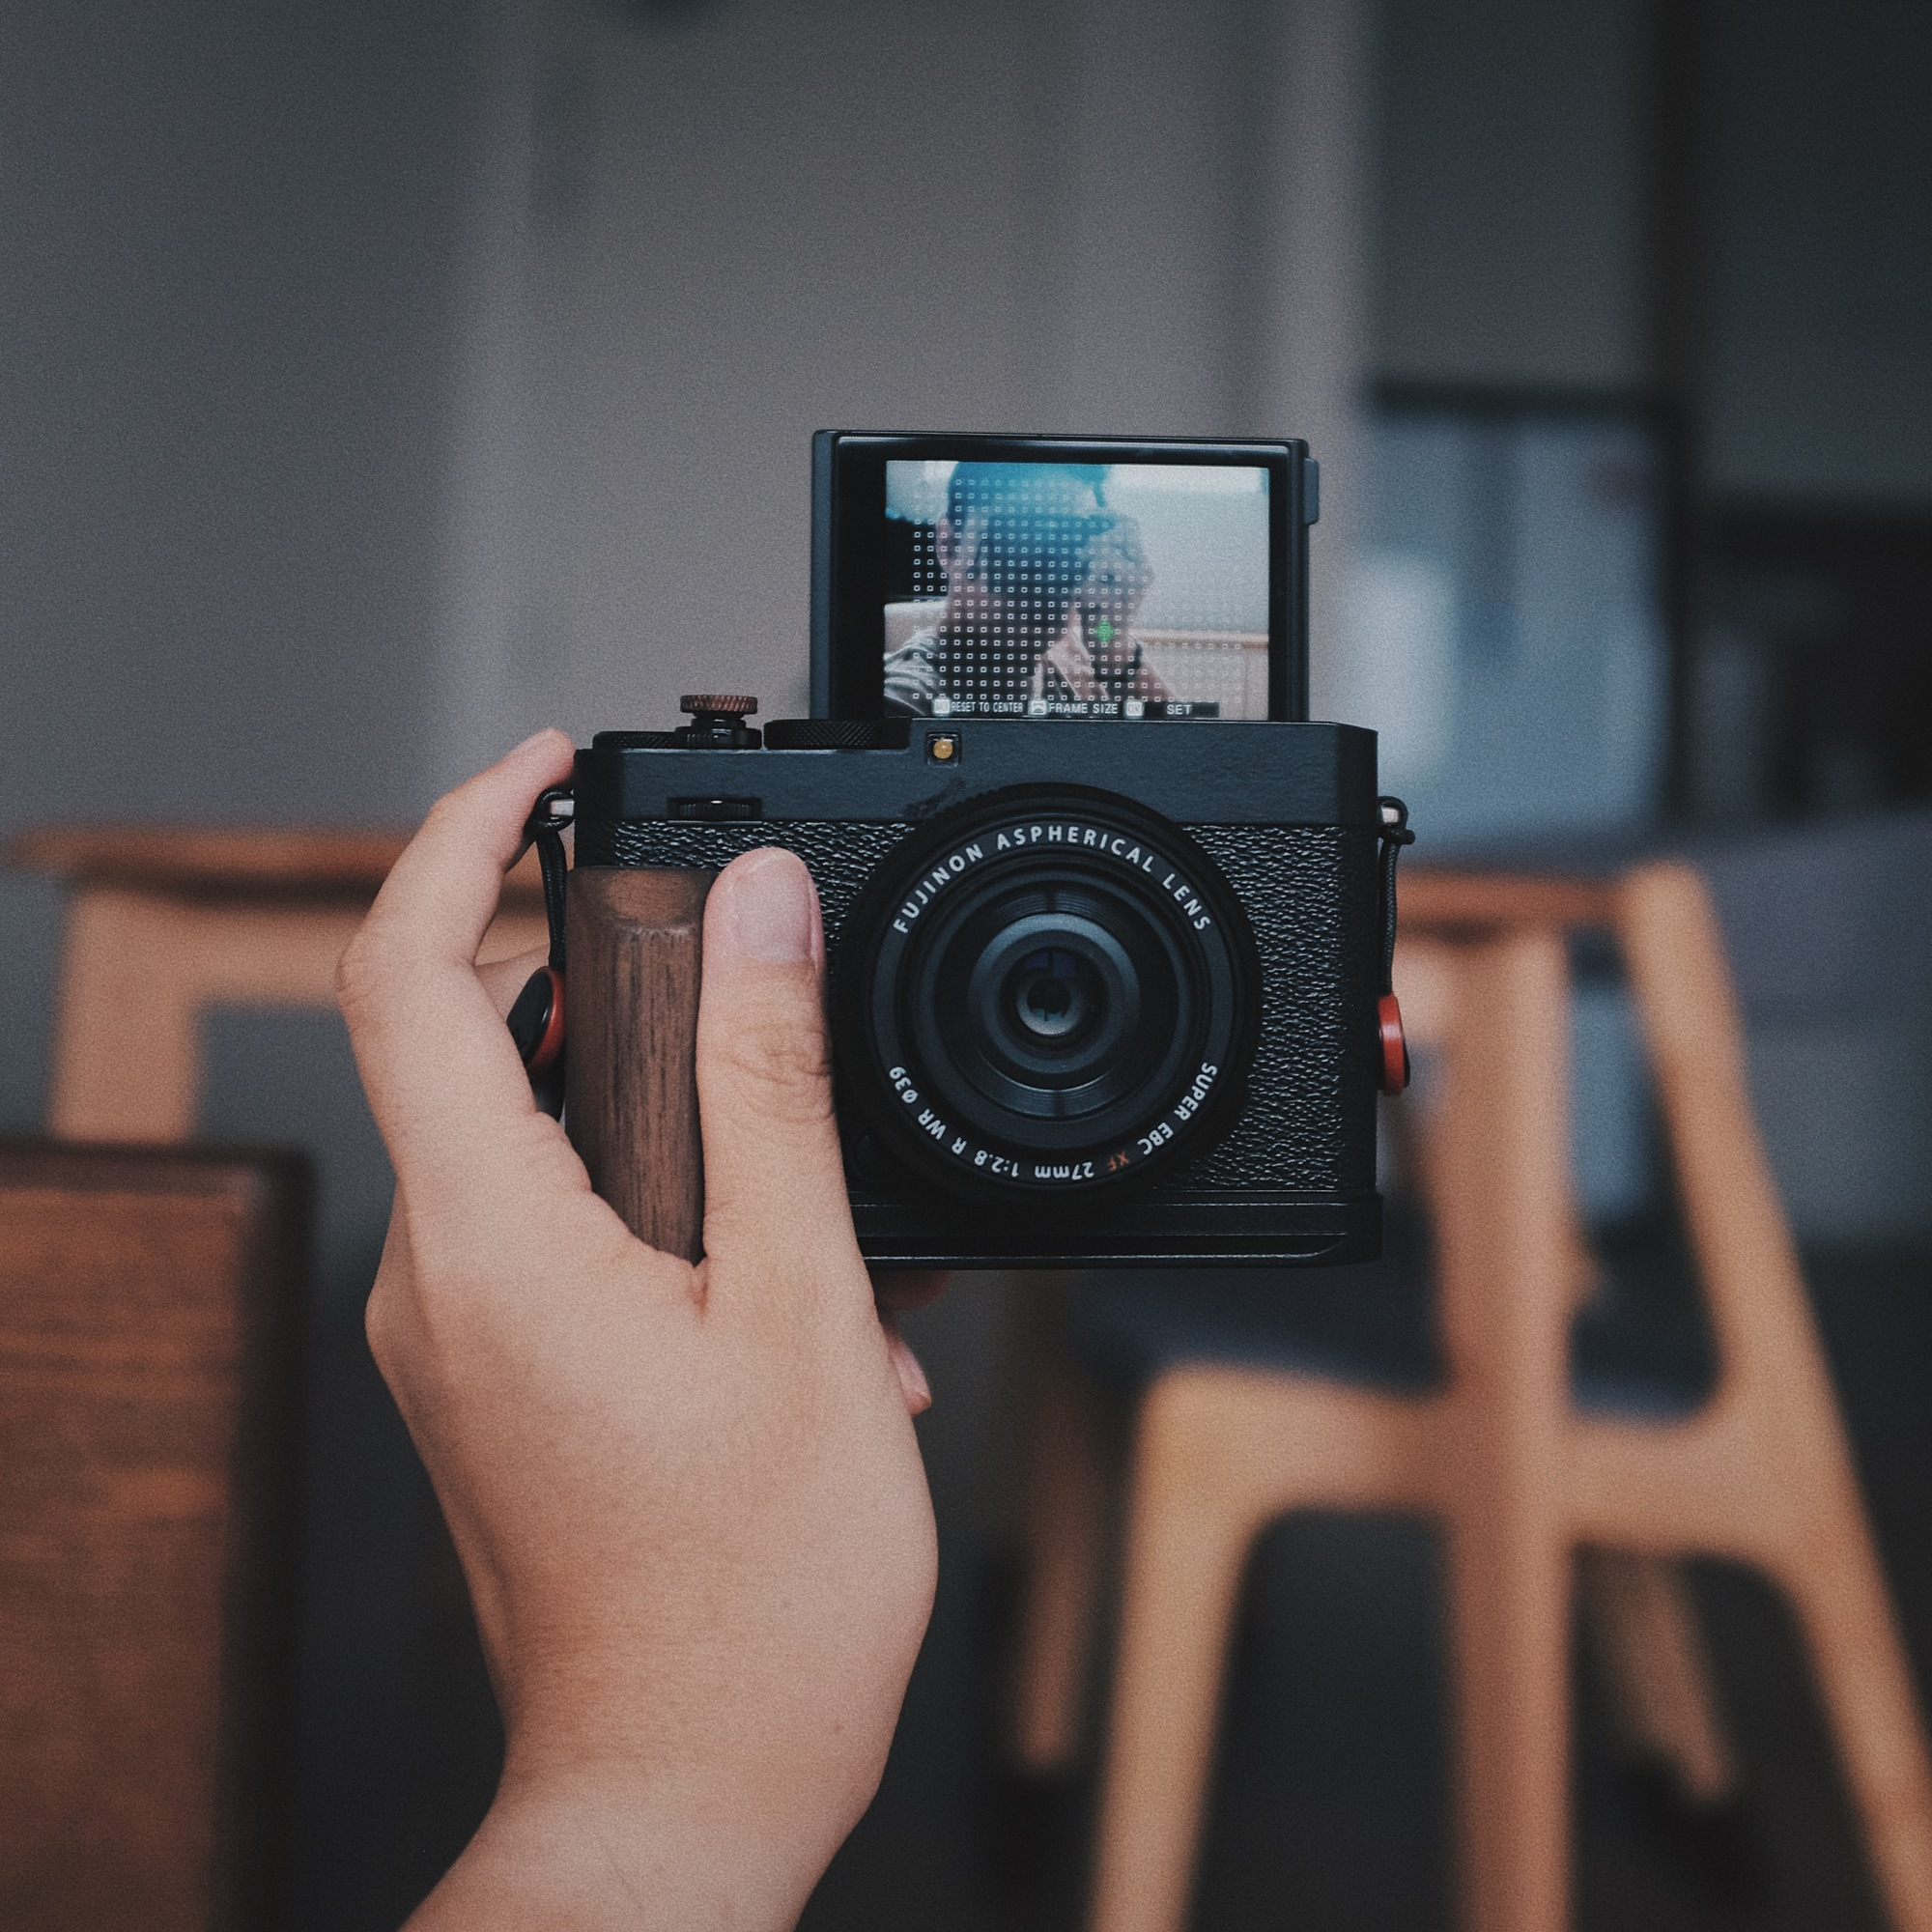
\includegraphics[width=\linewidth]{\envfinaldir/coverpic-prod.jpg}\par
            % \vskip 30pt
            \vfill

            \normalsize\rmfamily\scshape
            \copyright{} The Web Digest Project \hfill\large \envdatestr
        \end{center}
    \end{titlepage}
    % \restoregeometry
}
\newcommand{\simplehref}[1]{%
    \textcolor{blue!80!green}{\href{#1}{#1}}%
}
\renewcommand{\contentsname}{\center\Huge\sffamily\bfseries Contents\par\vskip 20pt}
\newcounter{ipartcounter}
\setcounter{ipartcounter}{0}
\newcommand{\ipart}[1]{
    % \vskip 20pt
    \clearpage
    \stepcounter{ipartcounter}
    \phantomsection
    \addcontentsline{toc}{chapter}{#1}
    % \begin{center}
    %     \Huge
    %     \sffamily\bfseries
    %     #1
    % \end{center}
    % \vskip 20pt plus 7pt
}
\newcounter{ichaptercounter}
\setcounter{ichaptercounter}{0}
\newcommand{\ichapter}[1]{
    % \vskip 20pt
    \clearpage
    \stepcounter{ichaptercounter}
    \phantomsection
    \addcontentsline{toc}{section}{\numberline{\arabic{ichaptercounter}}#1}
    \begin{center}
        \Huge
        \sffamily\bfseries
        #1
    \end{center}
    \vskip 20pt plus 7pt
}
\newcommand{\entrytitlefont}[1]{\subsection*{\raggedright\Large\sffamily\bfseries#1}}
\newcommand{\entryitemGeneric}[2]{
    % argv: title, url
    \parbox{\linewidth}{
        \entrytitlefont{#1}\par\vskip 5pt
        \footnotesize\ttfamily\mdseries
        \simplehref{#2}
    }\vskip 11pt plus 11pt minus 1pt
}
\newcommand{\entryitemGithub}[3]{
    % argv: title, url, desc
    \parbox{\linewidth}{
        \entrytitlefont{#1}\par\vskip 5pt
        \footnotesize\ttfamily\mdseries
        \simplehref{#2}\par\vskip 5pt
        \small\rmfamily\mdseries#3
    }\vskip 11pt plus 11pt minus 1pt
}
\newcommand{\entryitemAp}[3]{
    % argv: title, url, desc
    \parbox{\linewidth}{
        \entrytitlefont{#1}\par\vskip 5pt
        \footnotesize\ttfamily\mdseries
        \simplehref{#2}\par\vskip 5pt
        \small\rmfamily\mdseries#3
    }\vskip 11pt plus 11pt minus 1pt
}
\newcommand{\entryitemHackernews}[3]{
    % argv: title, hnurl, rawurl
    % \parbox{\linewidth}{
    %     \entrytitlefont{#1}\par\vskip 5pt
    %     \footnotesize\ttfamily\mdseries
    %     \simplehref{#3}\par
    %     \textcolor{black!50}{\href{#2}{#2}}
    % }\vskip 11pt plus 11pt minus 1pt
    \begin{minipage}{\linewidth}
            \entrytitlefont{#1}\par\vskip 5pt
            \footnotesize\ttfamily\mdseries
            \simplehref{#3}\par
            \textcolor{black!50}{\href{#2}{#2}}
    \end{minipage}\par\vskip 11pt plus 11pt minus 1pt
}







\begin{document}

\makeheader

\tableofcontents\clearpage




\ipart{Developers}
\ichapter{Hacker News}
\entryitemTwoLinks{Full Text Search of US Court records}{https://news.ycombinator.com/item?id=43731552}{https://www.judyrecords.com/}

\entryitemTwoLinks{15,000 lines of verified cryptography now in Python}{https://news.ycombinator.com/item?id=43731165}{https://jonathan.protzenko.fr/2025/04/18/python.html}

\entryitemTwoLinks{Judge Rules Blanket Search of Cell Tower Data Unconstitutional}{https://news.ycombinator.com/item?id=43730545}{https://www.404media.co/judge-rules-blanket-search-of-cell-tower-data-unconstitutional/}

\entryitemTwoLinks{Show HN: I made a Doom-like game fit inside a QR code}{https://news.ycombinator.com/item?id=43729683}{https://github.com/Kuberwastaken/backdooms}

\entryitemTwoLinks{A New ASN.1 API for Python}{https://news.ycombinator.com/item?id=43728279}{https://blog.trailofbits.com/2025/04/18/sneak-peek-a-new-asn.1-api-for-python/}

\entryitemTwoLinks{A Math Lesson From Hitler's Germany (2017)}{https://news.ycombinator.com/item?id=43728130}{https://undark.org/2017/02/01/math-lesson-hitlers-germany/}

\entryitemTwoLinks{Less Slow C++}{https://news.ycombinator.com/item?id=43727743}{https://github.com/ashvardanian/less\_slow.cpp}

\entryitemTwoLinks{IBM orders US sales to locate near customers, RTO for cloud staff, DEI purge}{https://news.ycombinator.com/item?id=43727727}{https://www.theregister.com/2025/04/18/ibm\_orders\_us\_sales\_staff/}

\entryitemTwoLinks{Walled Gardens Can Kill}{https://news.ycombinator.com/item?id=43726672}{https://aneesiqbal.ai/2025-04-18-walled-gardens-can-kill}

\entryitemTwoLinks{arXiv moving from Cornell servers to Google Cloud}{https://news.ycombinator.com/item?id=43726640}{https://info.arxiv.org/hiring/index.html}

\entryitemTwoLinks{Deafening Silence from the Cybersecurity Industry}{https://news.ycombinator.com/item?id=43726548}{https://www.forbes.com/sites/tonybradley/2025/04/16/deafening-silence-from-the-cybersecurity-industry/}

\entryitemTwoLinks{Defold: cross-platform game engine}{https://news.ycombinator.com/item?id=43726051}{https://defold.com}

\entryitemTwoLinks{AMP and why emails are not (and should never be) interactive}{https://news.ycombinator.com/item?id=43725865}{https://buttondown.com/blog/whatever-happened-to-amp-email}

\entryitemTwoLinks{I gave up on self-hosted Sentry (2024)}{https://news.ycombinator.com/item?id=43725815}{https://www.bugsink.com/blog/why-i-gave-up-on-self-hosted-sentry/}

\entryitemTwoLinks{Viral ChatGPT trend is doing 'reverse location search' from photos}{https://news.ycombinator.com/item?id=43725648}{https://techcrunch.com/2025/04/17/the-latest-viral-chatgpt-trend-is-doing-reverse-location-search-from-photos/}

\entryitemTwoLinks{Kagi Assistant is now available to all users}{https://news.ycombinator.com/item?id=43724941}{https://blog.kagi.com/assistant-for-all}

\entryitemTwoLinks{Why is Good Friday called Good Friday?}{https://news.ycombinator.com/item?id=43724870}{https://www.historyextra.com/period/general-history/good-friday-facts-why-called/}

\entryitemTwoLinks{Intuit, Owner of TurboTax, Wins Battle Against America's Taxpayers}{https://news.ycombinator.com/item?id=43724267}{https://prospect.org/power/2025-04-17-intuit-turbotax-wins-battle-against-taxpayers-irs-direct-file/}

\entryitemTwoLinks{DHL suspends B2C shipments over 800 USD until further notice}{https://news.ycombinator.com/item?id=43724123}{https://www.dhl.com/au-en/home/important-information/2025/shipments-to-the-united-states-with-a-customs-value-exceeding-usd-800.html}

\entryitemTwoLinks{ChatGPT now performs well at GeoGuesser}{https://news.ycombinator.com/item?id=43723408}{https://flausch.social/@piegames/114352447253793517}\ichapter{Phoronix}
\entryitemGeneric{\hskip 0pt{}Slightly Faster AES-XTS Performance For AVX-512 CPUs Expected With Linux 6.16}{https://www.phoronix.com/news/Linux-6.16-AES-XTS-AVX-512-Fast}

\entryitemGeneric{\hskip 0pt{}Initial Linux Gaming/Graphics Performance For The NVIDIA GeForce RTX 5060 Ti}{https://www.phoronix.com/review/nvidia-rtx-5060ti-linux-gaming}

\entryitemGeneric{\hskip 0pt{}Intel Xe Driver Adds Fan Speed Reporting For Linux 6.16, BMG Instability Being Debugged}{https://www.phoronix.com/news/Intel-Xe-Linux-6.16-Fan-Speeds}

\entryitemGeneric{\hskip 0pt{}GCC 15.1 Compiler Release Candidate For Testing, GCC 15.1.0 Potentially Next Week}{https://www.phoronix.com/news/GCC-15.1-RC-Released}

\entryitemGeneric{\hskip 0pt{}Fedora 43 Eyes Changing CMake's Default Generator From Make To Ninja}{https://www.phoronix.com/news/Fedora-43-Proposed-CMake-Ninja}

\entryitemGeneric{\hskip 0pt{}LVFS/Fwupd Is Hoping To Encourage More Hardware Vendors To Provide Financial Backing}{https://www.phoronix.com/news/LVFS-Needs-More-Funding}

\entryitemGeneric{\hskip 0pt{}Intel Compute Runtime 25.13.33276.16 Brings New Performance Tweaks, More Xe3 Bits}{https://www.phoronix.com/news/Intel-CR-25.13.33276.16}

\entryitemGeneric{\hskip 0pt{}Intel SST-TF Prepares For Future CPUs With More Cores}{https://www.phoronix.com/news/Intel-SST-TF-More-Than-256-Core}

\entryitemGeneric{\hskip 0pt{}Open-Source RADV Driver Begins Working To Improve AMD RDNA4 Ray-Tracing Performance}{https://www.phoronix.com/news/RADV-Aiming-Better-RDNA4-RT}\ichapter{Dribbble}
\entryitemGeneric{\hskip 0pt{}Case study: Educational Website on Space Pollution}{https://dribbble.com/shots/25914349-Case-study-Educational-Website-on-Space-Pollution}

\entryitemGeneric{\hskip 0pt{}Columbus Rapids®}{https://dribbble.com/shots/25915181-Columbus-Rapids}

\entryitemGeneric{\hskip 0pt{}UNIC // Mobile App}{https://dribbble.com/shots/25913185-UNIC-Mobile-App}

\entryitemGeneric{\hskip 0pt{}Cute Easter Bunny Mascot}{https://dribbble.com/shots/25914543-Cute-Easter-Bunny-Mascot}

\entryitemGeneric{\hskip 0pt{}Phantom concept with Widget}{https://dribbble.com/shots/25911511-Phantom-concept-with-Widget}

\entryitemGeneric{\hskip 0pt{}Crypto Widget}{https://dribbble.com/shots/25913330-Crypto-Widget}

\entryitemGeneric{\hskip 0pt{}Startup Branding for Holidu: visual identity, brand design}{https://dribbble.com/shots/25903662-Startup-Branding-for-Holidu-visual-identity-brand-design}

\entryitemGeneric{\hskip 0pt{}Mountains to Sea}{https://dribbble.com/shots/25910072-Mountains-to-Sea}

\entryitemGeneric{\hskip 0pt{}Cute Unicorn Mascot}{https://dribbble.com/shots/25909768-Cute-Unicorn-Mascot}

\entryitemGeneric{\hskip 0pt{}Logolounge Book 15 Entry - Client Work}{https://dribbble.com/shots/25909344-Logolounge-Book-15-Entry-Client-Work}

\entryitemGeneric{\hskip 0pt{}Forg Logo}{https://dribbble.com/shots/25910287-Forg-Logo}

\entryitemGeneric{\hskip 0pt{}Reindeer in Golden Light 🦌}{https://dribbble.com/shots/25905633-Reindeer-in-Golden-Light}

\entryitemGeneric{\hskip 0pt{}Altitude}{https://dribbble.com/shots/25902364-Altitude}

\entryitemGeneric{\hskip 0pt{}Logo Collection > Birds Volume 03}{https://dribbble.com/shots/25905911-Logo-Collection-Birds-Volume-03}

\entryitemGeneric{\hskip 0pt{}Automation builder - Wireframes}{https://dribbble.com/shots/25904187-Automation-builder-Wireframes}

\entryitemGeneric{\hskip 0pt{}Details - Amplemarket Logo \& Visual Identity}{https://dribbble.com/shots/25904732-Details-Amplemarket-Logo-Visual-Identity}

\entryitemGeneric{\hskip 0pt{}LogoLounge Book 15 Entry}{https://dribbble.com/shots/25904019-LogoLounge-Book-15-Entry}

\entryitemGeneric{\hskip 0pt{}FarmGirl Fresh®}{https://dribbble.com/shots/25905838-FarmGirl-Fresh}

\entryitemGeneric{\hskip 0pt{}Road Tripping}{https://dribbble.com/shots/25900418-Road-Tripping}

\entryitemGeneric{\hskip 0pt{}Lion sketches}{https://dribbble.com/shots/25898381-Lion-sketches}

\entryitemGeneric{\hskip 0pt{}Bloksy Logo Design - City, Colorful, Building, Construction}{https://dribbble.com/shots/25898764-Bloksy-Logo-Design-City-Colorful-Building-Construction}

\entryitemGeneric{\hskip 0pt{}Cute Shiba Catching a Ball}{https://dribbble.com/shots/25900210-Cute-Shiba-Catching-a-Ball}

\entryitemGeneric{\hskip 0pt{}Corti: Visual identity exploration}{https://dribbble.com/shots/25899331-Corti-Visual-identity-exploration}

\entryitemGeneric{\hskip 0pt{}Lume landing page interaction}{https://dribbble.com/shots/25898487-Lume-landing-page-interaction}


\ipart{Developers~~~~(zh-Hans)}
\ichapter{Solidot}
\entryitemGeneric{\hskip 0pt{}美国法官裁决 Google 非法垄断在线广告技术}{https://www.solidot.org/story?sid=81084}

\entryitemGeneric{\hskip 0pt{}Tor Browser 14.5 释出}{https://www.solidot.org/story?sid=81083}

\entryitemGeneric{\hskip 0pt{}Ubuntu 25.04 释出}{https://www.solidot.org/story?sid=81082}

\entryitemGeneric{\hskip 0pt{}数万年前人类或通过特制衣物和赭石防晒霜抵御强辐射}{https://www.solidot.org/story?sid=81081}

\entryitemGeneric{\hskip 0pt{}海豚因 PCB 污染而死亡风险上升}{https://www.solidot.org/story?sid=81080}

\entryitemGeneric{\hskip 0pt{}日本科学家发现可预防晕车的声音}{https://www.solidot.org/story?sid=81079}

\entryitemGeneric{\hskip 0pt{}天文学家发现一颗绕双星运行的行星}{https://www.solidot.org/story?sid=81078}

\entryitemGeneric{\hskip 0pt{}微软开发出超高效的能运行在 CPU 上的 AI 模型}{https://www.solidot.org/story?sid=81077}

\entryitemGeneric{\hskip 0pt{}《矮人要塞》售出了逾 100 万份拷贝}{https://www.solidot.org/story?sid=81076}

\entryitemGeneric{\hskip 0pt{}科学家演示用雨滴发电}{https://www.solidot.org/story?sid=81075}

\entryitemGeneric{\hskip 0pt{}天文学家发现了一颗可能有生命的行星}{https://www.solidot.org/story?sid=81074}

\entryitemGeneric{\hskip 0pt{}Google 宣布将逐步淘汰它使用的国家顶级域名}{https://www.solidot.org/story?sid=81073}

\entryitemGeneric{\hskip 0pt{}GoDaddy 错误关闭域名导致 Zoom 宕机}{https://www.solidot.org/story?sid=81072}

\entryitemGeneric{\hskip 0pt{}芯片未来将会越来越热}{https://www.solidot.org/story?sid=81071}

\entryitemGeneric{\hskip 0pt{}美国主要 AI 公司六成其创始人有移民背景}{https://www.solidot.org/story?sid=81070}

\entryitemGeneric{\hskip 0pt{}天文学家绘制星际冰地图}{https://www.solidot.org/story?sid=81069}

\entryitemGeneric{\hskip 0pt{}OpenAI 正在构建社交网络}{https://www.solidot.org/story?sid=81068}

\entryitemGeneric{\hskip 0pt{}苹果将使用英特尔处理器的 Mac mini 归类为过时产品}{https://www.solidot.org/story?sid=81067}

\entryitemGeneric{\hskip 0pt{}使用智能手机的老年人有较低的认知衰退率}{https://www.solidot.org/story?sid=81066}

\entryitemGeneric{\hskip 0pt{}Android 手机将设置三天不使用会自动重启}{https://www.solidot.org/story?sid=81065}\ichapter{V2EX}
\entryitemGeneric{\hskip 0pt{}[问与答] 想问下大家自己的项目在哪里管理的?希望一站式解决 git、需求、文档 几个需求}{https://www.v2ex.com/t/1126601}

\entryitemGeneric{\hskip 0pt{}[分享发现] 文案工作者必看!查找替换融入 AI,效率狂飙 1000\%!}{https://www.v2ex.com/t/1126600}

\entryitemGeneric{\hskip 0pt{}[问与答] 现在最快的效果还不错的开源 AI 生成图片模型是什么?}{https://www.v2ex.com/t/1126599}

\entryitemGeneric{\hskip 0pt{}[Chrome] DISCUZ 论坛登陆不上}{https://www.v2ex.com/t/1126597}

\entryitemGeneric{\hskip 0pt{}[问与答] 可以用 curl 重啟 tplink 路由器嗎?}{https://www.v2ex.com/t/1126596}

\entryitemGeneric{\hskip 0pt{}[酷工作] 寻前端开发(兼职、实习)一名}{https://www.v2ex.com/t/1126595}

\entryitemGeneric{\hskip 0pt{}[分享创造] nextjs 写一个关卡站来练手}{https://www.v2ex.com/t/1126594}

\entryitemGeneric{\hskip 0pt{}[分享创造] [不定更] 用 CLIPS 模拟生态}{https://www.v2ex.com/t/1126593}

\entryitemGeneric{\hskip 0pt{}[OpenAI] ChatGPT 网页端登录 要求输入手机号码。IOS 端不需要,只需输入游戏密码}{https://www.v2ex.com/t/1126592}

\entryitemGeneric{\hskip 0pt{}[编程] 常用大模型编程项目得分排名 04-19}{https://www.v2ex.com/t/1126591}

\entryitemGeneric{\hskip 0pt{}[职场话题] 一个 CTO 的深度思考}{https://www.v2ex.com/t/1126590}

\entryitemGeneric{\hskip 0pt{}[问与答] 约女生出来玩,对方总想叫朋友一起,是不是没戏了}{https://www.v2ex.com/t/1126589}

\entryitemGeneric{\hskip 0pt{}[问与答] cash APP 的钱可以直接转账到银行么?}{https://www.v2ex.com/t/1126588}

\entryitemGeneric{\hskip 0pt{}[分享创造] [测试邀请] 分享一个独立开发的部署工具 CelerBuild:只懂 shell 就能玩转,求试用和反馈!}{https://www.v2ex.com/t/1126585}

\entryitemGeneric{\hskip 0pt{}[微软] 微软网站是不是更新了}{https://www.v2ex.com/t/1126584}

\entryitemGeneric{\hskip 0pt{}[分享发现] chrome 扩展 Grabbit 打开框选的多个链接}{https://www.v2ex.com/t/1126583}

\entryitemGeneric{\hskip 0pt{}[NAS] 消费级非 ecc 内存使用 zfs 文件系统需要定时重启吗}{https://www.v2ex.com/t/1126582}

\entryitemGeneric{\hskip 0pt{}[分享创造] [网站自荐] Multiple URLs Opener 专业 URL 多开工具,支持 ``域名后缀多开'' 与 ``URL 列表多开'' 两种模式。域名后缀收藏分组、定时打开及历史记录等贴心功能,助你轻松应对各类批量访问场景}{https://www.v2ex.com/t/1126581}

\entryitemGeneric{\hskip 0pt{}[VXNA] 申请收录个人博客:缘生笔记}{https://www.v2ex.com/t/1126579}

\entryitemGeneric{\hskip 0pt{}[GitHub] github action 计费问题}{https://www.v2ex.com/t/1126577}

\entryitemGeneric{\hskip 0pt{}[问与答] windows 下 word 编辑文件变为临时文件问题}{https://www.v2ex.com/t/1126575}

\entryitemGeneric{\hskip 0pt{}[问与答] 求免费多端同步好一点的笔记软件}{https://www.v2ex.com/t/1126574}

\entryitemGeneric{\hskip 0pt{}[Apple] FileSentinel:一款文件监视器,自动监控 .zsh\_history 等文件并保存记录,帮助你轻松搜索和回顾最近的终端命令,再也不怕忘记复杂命令}{https://www.v2ex.com/t/1126573}

\entryitemGeneric{\hskip 0pt{}[分享创造] 手搓了一个生成即梦文字``提示词秘籍''的生成页}{https://www.v2ex.com/t/1126572}

\entryitemGeneric{\hskip 0pt{}[程序员] 像这种自媒体平台查权重,这种接口都是怎么弄到的啊?}{https://www.v2ex.com/t/1126570}

\entryitemGeneric{\hskip 0pt{}[问与答] Manus 都要排队了?!什么情况?算力不够?用户暴增?}{https://www.v2ex.com/t/1126568}

\entryitemGeneric{\hskip 0pt{}[问与答] 那个能做风格迁移,能 p 图的 gpt-4o 在哪个二手平台能用啊}{https://www.v2ex.com/t/1126567}

\entryitemGeneric{\hskip 0pt{}[问与答] 大家有对媒体文件管理的需求吗?比如经营公众号或者对相册备份。 除了网盘还有好用的类似多媒体文件管理系统吗?限于网页端吧。}{https://www.v2ex.com/t/1126566}

\entryitemGeneric{\hskip 0pt{}[问与答] 订阅了 cursor 还需要 v0 吗?}{https://www.v2ex.com/t/1126565}

\entryitemGeneric{\hskip 0pt{}[程序员] 任何带``取消''键的表单都想按按看}{https://www.v2ex.com/t/1126564}

\entryitemGeneric{\hskip 0pt{}[MacBook Pro] 突然发现, Mac 连着 iPhone 热点的时候,如果打开 iPhone 镜像,热点就会断掉…}{https://www.v2ex.com/t/1126560}

\entryitemGeneric{\hskip 0pt{}[NAS] 求推荐 Nas,可能我的要求比较刁钻}{https://www.v2ex.com/t/1126558}

\entryitemGeneric{\hskip 0pt{}[推广] 大家好!我们是霓虹比特(NeonBit 团队),我们即将推出,出海社媒营销 AI+ 工具 - SnapVee AI}{https://www.v2ex.com/t/1126557}

\entryitemGeneric{\hskip 0pt{}[Markdown] 有什么支持原地渲染的 Markdown 编辑器,并且非常容易支持导出原始 Markdown 的?}{https://www.v2ex.com/t/1126556}

\entryitemGeneric{\hskip 0pt{}[问与答] 关于 Infini 狗卡的使用}{https://www.v2ex.com/t/1126555}

\entryitemGeneric{\hskip 0pt{}[JavaScript] 🚀 让网页字体调整更轻松!来试试我写的 NiceFont 脚本呗 -。-'🎉}{https://www.v2ex.com/t/1126554}

\entryitemGeneric{\hskip 0pt{}[San Francisco] VAT Calculator}{https://www.v2ex.com/t/1126553}

\entryitemGeneric{\hskip 0pt{}[WordPress] 主题巴巴彻底跑路了}{https://www.v2ex.com/t/1126552}

\entryitemGeneric{\hskip 0pt{}[酷工作] 字节跳动「芯片团队 」大量研发岗位等你来!}{https://www.v2ex.com/t/1126551}

\entryitemGeneric{\hskip 0pt{}[宽带症候群] 神奇的 OBS 更新触发断网机制,绷不住了}{https://www.v2ex.com/t/1126550}

\entryitemGeneric{\hskip 0pt{}[程序员] 如何用代码破解打招呼难题?}{https://www.v2ex.com/t/1126549}

\entryitemGeneric{\hskip 0pt{}[Solana] 部署 Solana 归档节点需要什么样的配置?}{https://www.v2ex.com/t/1126548}

\entryitemGeneric{\hskip 0pt{}[问与答] lenny 订阅已经没法获得 Cursor 年会了吗}{https://www.v2ex.com/t/1126547}

\entryitemGeneric{\hskip 0pt{}[职场话题] 今天领大礼包了}{https://www.v2ex.com/t/1126546}

\entryitemGeneric{\hskip 0pt{}[酷工作] 继续招聘,欢迎投递~[TOP1 券商] [社招-深圳] 交易结算系统研发工程师}{https://www.v2ex.com/t/1126545}

\entryitemGeneric{\hskip 0pt{}[问与答] 要做一个视频网站储存成本和流量成本要多少(用 cloudflare 的 stream 以及 R2)?}{https://www.v2ex.com/t/1126544}

\entryitemGeneric{\hskip 0pt{}[程序员] 开源 get-cookie-httponly 万能 Cookie 获取工具,突破 httponly 限制!}{https://www.v2ex.com/t/1126543}

\entryitemGeneric{\hskip 0pt{}[程序员] AI 编码,有什么 mcp 推荐吗?}{https://www.v2ex.com/t/1126542}

\entryitemGeneric{\hskip 0pt{}[WireGuard] wireguard 内网通讯的延迟大概是多少}{https://www.v2ex.com/t/1126540}

\entryitemGeneric{\hskip 0pt{}[程序员] 有没有大佬了解机器学习的 mlops 框架或者平台}{https://www.v2ex.com/t/1126539}


\ipart{Generic News}







\clearpage
\leavevmode\vfill
\footnotesize

Copyright \copyright{} 2023-2025 Neruthes and other contributors.

This document is published with CC BY-NC-ND 4.0 license.

The entries listed in this newsletter may be copyrighted by their respective creators.

This newsletter is generated by the Web Digest project.

The newsletters are also delivered via Telegram channel \CJKunderline{\href{https://t.me/webdigestchannel}{https://t.me/webdigestchannel}}.\\
RSS feed is available at \CJKunderline{\href{https://webdigest.pages.dev/rss.xml}{https://webdigest.pages.dev/rss.xml}}.

This newsletter is available in PDF at
\CJKunderline{\href{https://webdigest.pages.dev/}{https://webdigest.pages.dev/}}.

The source code being used to generate this newsletter is available at\\
\CJKunderline{\href{https://github.com/neruthes/webdigest}{https://github.com/neruthes/webdigest}}.

This newsletter is also available in
\CJKunderline{\href{http://webdigest.pages.dev/readhtml/\envyear/WebDigest-20250419.html}{HTML}} and
\CJKunderline{\href{https://github.com/neruthes/webdigest/blob/master/markdown/\envyear/WebDigest-20250419.md}{Markdown}}.


\coverpic{https://unsplash.com/photos/cameras-and-accessories-are-neatly-arranged-on-a-tray-BtLDSIhhYwQ}{Grigorii Shcheglov}


\end{document}
